

The success of a mixed finite element formulation crucially depends on a proper choice of the local interpolations of the velocity and the pressure. 

%........................................................................................
\subsubsection{The compatibility condition (or LBB condition, or inf-sup condition)}
\index{general}{LBB} \index{general}{Optimal Rate}

WARNING: I am not comfortable writing about this topic. What follows is a rough attempt at making sense of it.


The Lady{\v z}henskaya-Babu{\v s}ka-Brezzi (LBB) condition is a sufficient 
condition for a saddle point problem to have a unique solution.
For saddle point problems coming from the Stokes equations, 
many discretizations are unstable, giving rise to artifacts such as spurious oscillations. 
The LBB condition gives criteria for when a discretization of a saddle point problem is stable. 
It also assures convergence at the optimal rate. 

Bochev \& Gunzburger \cite{bogu09} state: "
The terminology “LBB” originates from the facts that this condition was first explicitly discussed
in the finite element setting for saddle point problems by Brezzi \cite{brez74} and that it is a special case of
the general weak-coercivity condition first discussed for finite element methods by Babu{\v s}ka
\cite{babu71} and that, in the continuous setting of the Stokes equation, this condition was first proved to
hold by Ladyzhenskaya; see \cite{lady69}."

Unfortunately, to quote Donea \& Huerta \cite{dohu03}: 
"In the finite element context, it is by no means easy to prove whether or not a given
velocity-pressure pair satisfies the LBB compatibility condition."
Elman et al state: "[...] Choosing spaces for which the discrete inf-sup condition holds
and is a delicate matter, and seemingly natural choices of velocity and pressure approximation
do not work. [...] In general, care must be taken to make the velocity space 
rich enough compared to the pressure space."

The LBB condition, or inf-sup condition can be proven in different ways, and standard techniques have been designed
as listed in Boffi et al (2008) \cite{bobf08}.

%p129
Elman et al \cite{elsw} state that "The inf-sup condition is a sufficient condition for the pressure to be unique up
to  constant in the case of an enclosed flow." This can also be proven for other boundary conditions.
This approach, based on the macro-element technique \cite{sten90} is explored in Appendix \ref{app:Gel}.


It can be shown that, provided the kernel (null space) of matrix $\G$ is zero,
the Stokes matrix is non-singular, that is $\vec{\cal V}$ and $\vec{\cal P}$ 
are uniquely defined, and the Schur complement matrix $\SSS$ is positive definite. 
Simply put, taking $\vec{\cal V}=\vec{0}$ in the discretised Stokes system 
without body forces yields $\G \cdot \vec{\cal P}=\vec{0}$ and implies
that any pressure solution is only unique up to the null space of the matrix $\G$.

We know that the Schur complement matrix $\SSS$ is positive definite if and only if all of its eigenvalues are positive.
One could then (numerically) compute the eigenvalues of $\SSS$ and check that these are indeed strictly positive
to show that $\SSS$ is pos def. 

%Since $\SSS$ is trivially symmetric (because $\K$ is symmetric), then 

Another way is to see that $\SSS$ is positive definite only if $\text{ker}(\G)=\{0\}$.
Again to quote Donea \& Huerta \cite{dohu03}: "If this is the case, the partitioned Stokes matrix  
is non-singular and delivers uniquely defined velocity and pressure fields. If this is not the case, a
stable and convergent velocity field might be obtained, but the pressure field is likely
to present spurious and oscillatory results." 
Note that in the case of the $Q_1 \times P_0$ element it has been shown that the multiple families of 
checkboard pressure modes actually lie in the kernel of $\G$. \cite{XXXXsani}

One could then also numerically compute the Ker of G?

\vspace{.4cm}

LBB means velocity and pressure spaces yield uniquely defined vel and p solutions. 
is proving ker(G)=0 enough? is proving S (S)PD enough ?




%........................................................................................
\subsubsection{Families}
\index{general}{Taylor-Hood}

The family of \underline{Taylor-Hood} finite element spaces on triangular/tetrahedral 
grids is given by $P_k \times P_{k-1}$ with $k\geq 2$, 
and on quadrilateral/hexahedral grids by $Q_k \times Q_{k-1}$ with $k\geq 2$.
This means that the pressure is then approximated by continuous functions. 

These finite elements are very popular, in particular the pairs for $k=2$, i.e.
$Q_2\times Q_1$ and $P_2\times P_1$.
The reason why $k\geq 2$ comes from the fact that the 
$Q_1 \times Q_0$ (i.e. $Q_1 \times P_0$) and $P_2\times P_1$
are not stable elements (they are not inf-sup stable). 

\begin{remark}
Note that a similar element to $Q_2 \times Q_1$ has been proposed
and used succesfully used \cite{taho73,hota74}: it is denoted by $Q_2^{(8)} \times Q_1$ 
since the center node ('$x^2y^2$') and its associated degrees of freedom have been removed. It 
has also been proved to be LBB stable. 
\end{remark}


The \underline{Raviart-Thomas} family\todo{find literature} on triangles and quadrilaterals.

%........................................................................................
\subsubsection{The bi/tri-linear velocity - constant pressure element ($Q_1\times P_0$)}

\begin{minipage}[t]{0.5\textwidth}
\begin{flushright} {\tiny {\color{gray} (tikz\_q1p0.tex)}} \end{flushright}
%~~~~~~~~~~~~~~~~~~~~~~~~~~~~~~~~~~~~~~~~~~~~~~~~~~~~~~~~~~~~~~~~~~~~~~~~~~~~~~~~~~~~~~~~~~~~~~~~~~

\begin{tikzpicture}
%\draw[fill=gray!23,gray!23](0,0) rectangle (5,5);
%\draw[step=0.5cm,gray,very thin] (0,0) grid (4,4); %background grid
\draw[thick] (1,1) -- (3,1.2) -- (2.7,3) -- (1.1,3.1) -- cycle;  
\node[] at (0.8,0.8) {0};
\node[] at (3.2,1) {1};
\node[] at (2.9,3.1) {2};
\node[] at (0.9,3.2) {3};
\draw[violet] (1.9,2.075) circle (4pt);
\draw[black,fill=teal] (1,1)   circle (2pt);
\draw[black,fill=teal] (3,1.2)  circle (2pt);
\draw[black,fill=teal] (2.7,3)  circle (2pt);
\draw[black,fill=teal] (1.1,3.1) circle (2pt);
\draw[black,fill=teal] (3.1,0.2) circle (2pt); 
\node[] at (3.4,0.2) {$\vec\upnu$};
\draw[violet] (4.1,0.2) circle (4pt); 
\node[] at (4.4,0.2) {$p$};
\node[] at (2.5,4.5) {4 vel. nodes, 1 press. node};
\end{tikzpicture}

\end{minipage}
\begin{minipage}[t]{0.5\textwidth}

\begin{tikzpicture}
%\draw[fill=gray!23,gray!23](0,0) rectangle (5,5);
%\draw[step=0.25cm,gray,very thin] (0,0) grid (5,4); %background grid
\draw[thick] (1,0.5) -- (3.25,0.75) -- (3,3) -- (0.5,2.5) -- cycle; %1-2-6-5
\draw[thick] (3.25,0.75) -- (4,1.5) -- (4.25,3.75) -- (3,3) -- cycle; %2-3-7-6
\draw[thick] (0.5,2.5) -- (3,3) -- (4.25,3.75) -- (1.75,3.5) -- cycle; %5-6-7-4
\draw[thin]   (1,0.5) -- (2,1.75) -- (1.75,3.5) -- (0.5,2.5)   --cycle; % 1-0-4-5 
\draw[thin] (2,1.75) -- (4,1.5); 
%\node[] at (0.8,0.8) {0};
%\node[] at (3.2,1) {1};
%\node[] at (2.9,3.1) {2};
%\node[] at (0.9,3.2) {3};
\draw[violet] (2.5,2.) circle (4pt);
\draw[black,fill=teal] (1,0.5)   circle (2pt);
\draw[black,fill=teal] (3.25,0.75)   circle (2pt);
\draw[black,fill=teal] (3,3)   circle (2pt);
\draw[black,fill=teal] (0.5,2.5)   circle (2pt);
\draw[black,fill=teal] (1.75,3.5)  circle (2pt);
\draw[black,fill=teal] (4.25,3.75)  circle (2pt);
\draw[black,fill=teal] (4,1.5) circle (2pt);
\draw[black,fill=teal] (2,1.75) circle (2pt);
\draw[black,fill=teal] (3.1,0.2) circle (2pt); 
\node[] at (3.4,0.2) {$\vec\upnu$};
\draw[violet] (4.1,0.2) circle (4pt); 
\node[] at (4.4,0.2) {$p$};
\node[] at (2.5,4.5) {8 vel. nodes, 1 press. node};
\end{tikzpicture}

\end{minipage}

discussed in example 3.71 of \cite{john16}

However simple it may look, the \index{general}{$Q_1 \times P_0$} element is 
one of the hardest elements to analyze and many questions are still open about its properties. 
The element does not satisfy the inf-sup condition \cite{hugh}p211. 
In \cite{grsa} it is qualified as follows: slightly unstable but highly usable. 

The $Q_1 \times P_0$ mixed approximation is the lowest order conforming approximation 
method defined on a rectangular grid. It also happens to be the most famous example 
of an unstable mixed approximation method.
\cite[p235]{elsw}.

This element is discussed in \cite{fort81}, \cite{fofo85} and in \cite{pisa85} 
in the context of multigrid use.

This element is plagued by so-called pressure checkerboard modes which
have been thoroughly analysed \cite{grsi94}, \cite{chpc95}, \cite{sagl81a,sagl81b}.
These can be filtered out \cite{chpc95}. Smoothing techniques are also discussed in \cite{legs79}.

\Literature \cite{fobo90}\cite{grle85}\cite{leru86}



%----------------------------------------------------------------------
\subsubsection{The bi/tri-quadratic velocity - discontinuous linear pressure element ($Q_2 \times P_{-1}$)}

This element is crowned "probably the most accurate 2D element" in Gresho \& Sani's book \cite{grsa}.

It is characterised by piecewise Biquadratic velocities, 
and piecewise linear discontinuous polynomial pressure. 
The element satisfies the inf-sup condition, see page 211 of Hughes \cite{hugh}, or p138 of Elman et al
\cite{elsw}.
It is used in van de Vosse et al (1989) \cite{vavs89} for steady laminar flowin a curved tube. 
See Boffi \& Gastaldi (2002) \cite{boga02} 
for the two possible choices for the definition of the pressure space..
This element is mentioned in Kaus (2010) \cite{kaus10} and Pelletier et al (1989) \cite{pefc89} 
and it is  used in Frehner (2014) \cite{freh14} to study 3D fold growth rates 
(see online supplementary material) and in Schmalholtz (2008) \cite{schm08}.

Note that the serendipity version of this pair, i.e. $Q_2^{(20)}\times P_{-1}$ is also LBB stable
as shown in p180 of Reddy \cite{reddybook2}.

This element is implemented in Stone 76. 

\begin{center}
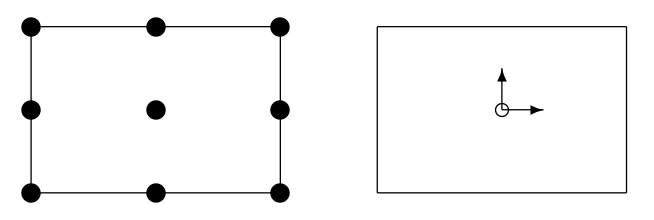
\includegraphics[width=6cm]{images/q2pm1/q2pm1}
\end{center}


%----------------------------------------------------------------------
\subsubsection{The bi/tri-quadratic velocity - bi/tri-linear pressure element ($Q_2 \times Q_1$)}
\label{ss:pairq2q1}

\begin{minipage}[t]{0.5\textwidth}
\begin{flushright} {\tiny {\color{gray} (tikz\_q2q1.tex)}} \end{flushright}
%~~~~~~~~~~~~~~~~~~~~~~~~~~~~~~~~~~~~~~~~~~~~~~~~~~~~~~~~~~~~~~~~~~~~~~~~~~~~~~~~~~~~~~~~~~~~~~~~~~

%\begin{center}
\begin{tikzpicture}
%\draw[fill=gray!23,gray!23](0,0) rectangle (5,5);
%\draw[step=0.5cm,gray,very thin] (0,0) grid (4,4); %background grid
\draw[thick] (1,1) -- (3,1.2) -- (2.7,3) -- (1.1,3.1) -- cycle;  
\node[] at (0.7,0.8) {0};
\node[] at (3.3,1) {1};
\node[] at (3,3.1) {2};
\node[] at (0.8,3.2) {3};
\draw[black,fill=teal] (1,1)     circle (2pt); \draw[violet] (1,1) circle (4pt);
\draw[black,fill=teal] (3,1.2)   circle (2pt); \draw[violet] (3,1.2) circle (4pt);
\draw[black,fill=teal] (2.7,3)   circle (2pt); \draw[violet] (2.7,3) circle (4pt);
\draw[black,fill=teal] (1.1,3.1) circle (2pt); \draw[violet] (1.1,3.1) circle (4pt);
\draw[black,fill=teal] (2,1.1) circle (2pt) ; \node[] at (2,0.8) {4};
\draw[black,fill=teal] (2.85,2.1) circle (2pt) ; \node[] at (3.1,2.1) {5};
\draw[black,fill=teal] (1.9,3.05) circle (2pt) ; \node[] at (1.9,3.3) {6};
\draw[black,fill=teal] (1.05,2.05) circle (2pt) ; \node[] at (0.8,2) {7};
\draw[black,fill=teal] (1.9,2.075) circle (2pt) ; \node[] at (2.1,2) {8};
\draw[black,fill=teal] (3.1,0.2) circle (2pt); 
\node[] at (3.4,0.2) {$\vec\upnu$};
\draw[violet] (4.1,0.2) circle (4pt); 
\node[] at (4.4,0.2) {$p$};
\node[] at (2.5,4.5) {9 vel. nodes, 4 press. nodes};
\end{tikzpicture}
%\end{center}

\end{minipage}
\begin{minipage}[t]{0.5\textwidth}



%\begin{center}
\begin{tikzpicture}
%\draw[fill=gray!23,gray!23](0,0) rectangle (5,5);
%\draw[step=0.5cm,gray,very thin] (0,0) grid (5,4); %background grid
\draw[thick] (1,0.5) -- (2,0.55) --(3.25,0.75) -- (3,3) -- (0.5,2.5) -- cycle; %1-9-2-6-5
\draw[thick] (3.25,0.75) -- (3.6,1.05) -- (4,1.5) -- (4.25,3.75) -- (3,3) -- cycle; %2-10-3-7-6
\draw[thick] (0.5,2.5) -- (3,3) -- (4.25,3.75) -- (1.75,3.5) -- (1.1,3.1) -- cycle; %5-6-7-4-13
\draw[thin]   (1,0.5) -- (1.5,1.25) -- (2,1.75) -- (1.75,3.5) -- (1.1,3.1) -- (0.5,2.5) --cycle; % 1-8-0-4-5-13 
\draw[thin] (2,1.75) -- (3,1.75) -- (4,1.5); %0-11-3
%pressure nodes
\draw[violet] (2,1.75) circle (4pt); % 0 
\draw[violet] (1,0.5) circle (4pt); % 1 
\draw[violet] (3.25,0.75) circle (4pt); % 2 
\draw[violet] (4,1.5) circle (4pt); % 3 
\draw[violet] (1.75,3.5) circle (4pt); % 4 
\draw[violet] (0.5,2.5) circle (4pt); % 5 
\draw[violet] (3,3) circle (4pt); % 6 
\draw[violet] (4.25,3.75) circle (4pt); % 7 
%velocity nodes
\draw[black,fill=teal] (1,0.5)   circle (2pt);
\draw[black,fill=teal] (3.25,0.75)   circle (2pt);
\draw[black,fill=teal] (3,3)   circle (2pt);
\draw[black,fill=teal] (0.5,2.5)   circle (2pt);
\draw[black,fill=teal] (1.75,3.5)  circle (2pt);
\draw[black,fill=teal] (4.25,3.75)  circle (2pt);
\draw[black,fill=teal] (4,1.5) circle (2pt);
\draw[black,fill=teal] (2,1.75) circle (2pt);
\draw[black,fill=teal] (1.5,1.25) circle (2pt); % 8 
\draw[black,fill=teal] (2,0.55) circle (2pt); % 9 
\draw[black,fill=teal] (3.6,1.05) circle (2pt); % 10
\draw[black,fill=teal] (3,1.75) circle (2pt); % 11
\draw[black,fill=teal] (0.75,1.5) circle (2pt); % 12
\draw[black,fill=teal] (1.1,3.1) circle (2pt); % 13
\draw[black,fill=teal] (0.75,1.5) circle (2pt); % 18
\draw[black,fill=teal] (2.7,1.1) circle (2pt); % 21
\draw[black,fill=teal] (3.6,3.35) circle (2pt); % 21
\draw[black,fill=teal] (3.,3.62) circle (2pt); % 21
\draw[black,fill=teal] (4.12,2.6) circle (2pt); % 21
\draw[black,fill=teal] (1.89,2.5) circle (2pt); % 21
\draw[black,fill=teal] (1.75,2.75) circle (2pt); % 21
\draw[black,fill=teal] (3.12,1.9) circle (2pt); % 21
\draw[black,fill=teal] (3.6,2.2) circle (2pt); % 21
\draw[black,fill=teal] (1.25,2.1) circle (2pt); % 21
\draw[black,fill=teal] (2.4,3.2) circle (2pt); % 21
\draw[black,fill=teal] (2.5,2.5) circle (2pt); % 21

% legend
\draw[black,fill=teal] (3.1,0.2) circle (2pt); \node[] at (3.4,0.2) {$\vec\upnu$};
\draw[violet] (4.1,0.2) circle (4pt); 
\node[] at (4.4,0.2) {$p$};
\node[] at (2.5,4.5) {27 vel. nodes, 8 press. nodes};
\end{tikzpicture}
%\end{center}


\end{minipage}


In \cite{grsa} Gresho \& Sani write that in their opinion $div(\vec v)=0$ is not strong enough.

This element, implemented in penalised form, is discussed in \cite{been79} and the follow-up paper \cite{been80}. CHECK

Biquadratic velocities, bilinear pressure. See Hood and Taylor. The element satisfies the inf-sup condition \cite{hugh}p215. 

\begin{center}
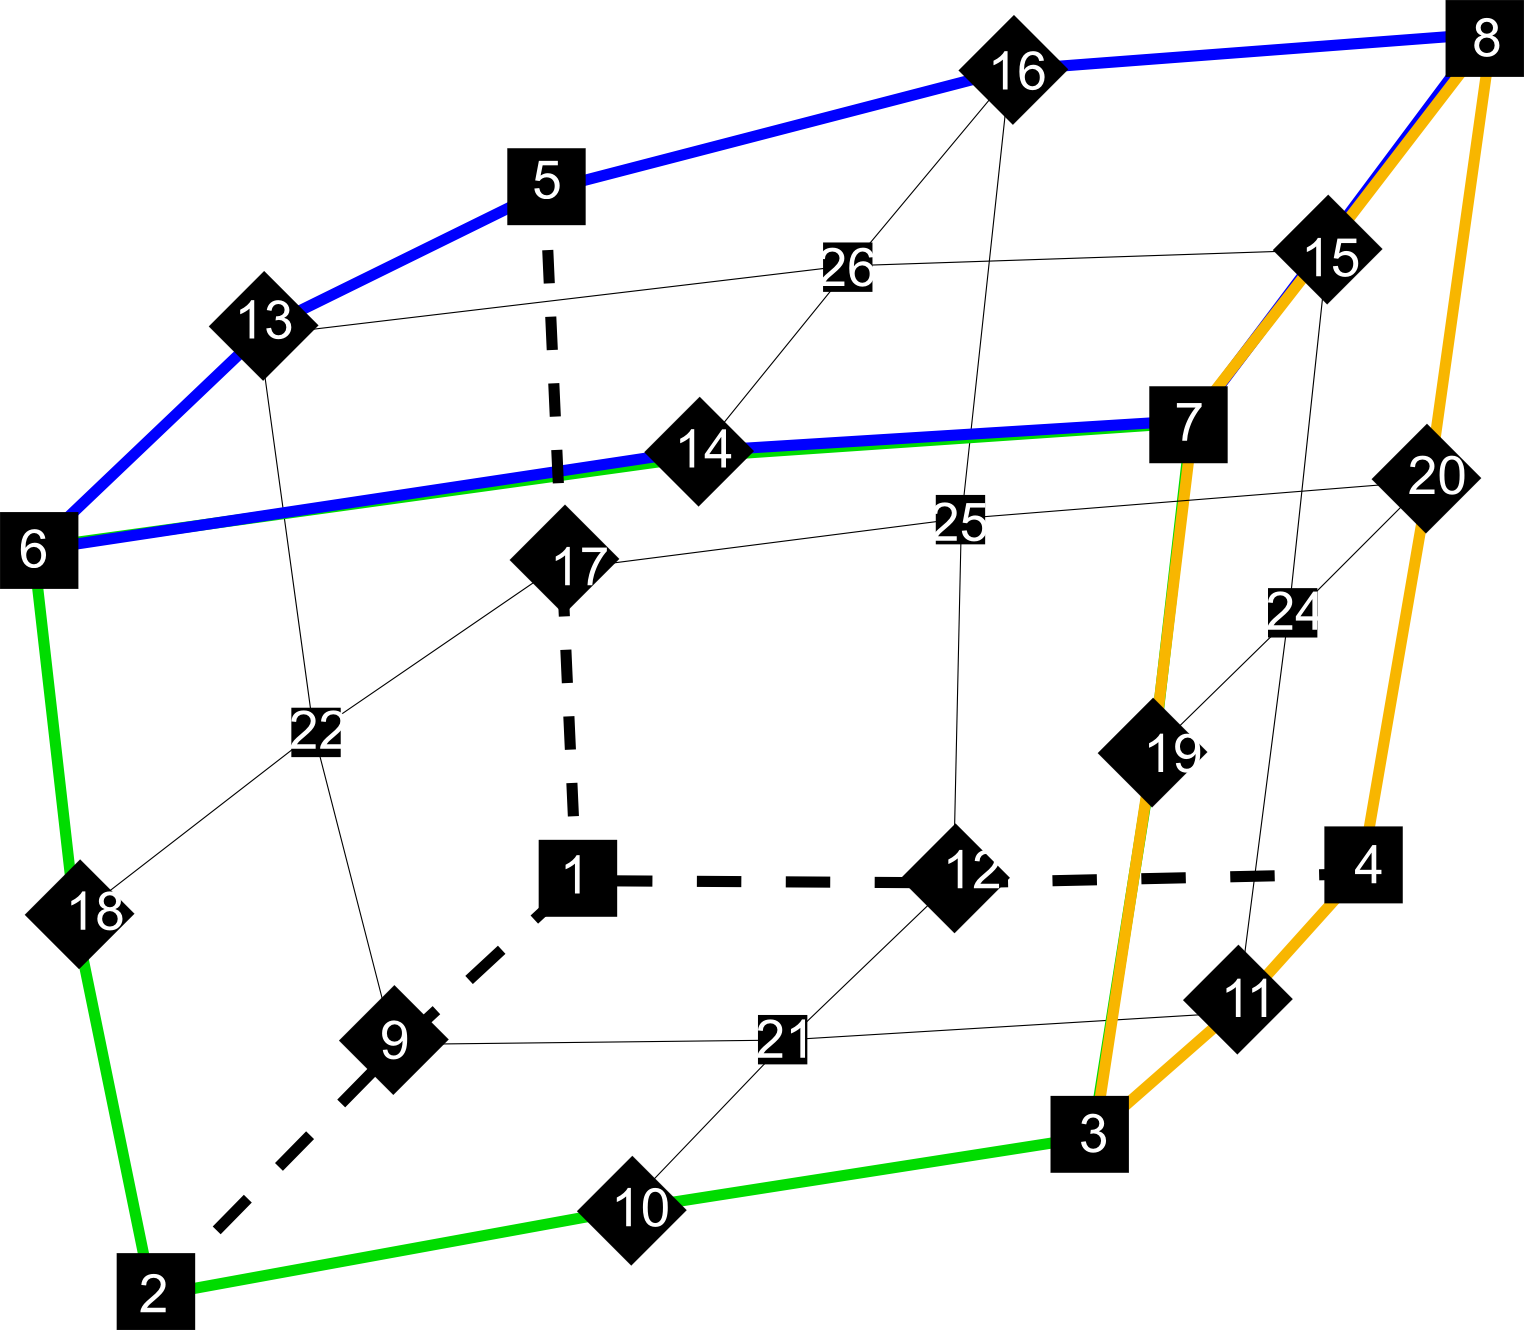
\includegraphics[width=6cm]{images/q2q1/q2numering}
\end{center}

%----------------------------------------------------------------------
\subsubsection{The stabilised bi/tri-linear velocity -  constant pressure element ($Q_1\times P_0$-stab)}

\Literature: \cite{sike90,vibo92,kesi92,qizh07,lisi12,chco01,chri02}

%----------------------------------------------------------------------
\subsubsection{The stabilised bi/tri-linear velocity -  bi/tri-linear pressure element ($Q_1\times Q_1$-stab)}

\begin{minipage}[t]{0.5\textwidth}

\begin{center}
\begin{tikzpicture}
%\draw[fill=gray!23,gray!23](0,0) rectangle (5,5);
%\draw[step=0.5cm,gray,very thin] (0,0) grid (4,4); %background grid
\draw[thick] (1,1) -- (3,1.2) -- (2.7,3) -- (1.1,3.1) -- cycle;  
\node[] at (0.8,0.8) {0};
\node[] at (3.2,1)   {1};
\node[] at (2.9,3.1) {2};
\node[] at (0.9,3.2) {3};
\draw[black,fill=teal] (1,1)     circle (2pt); \draw[violet] (1,1) circle (4pt);
\draw[black,fill=teal] (3,1.2)   circle (2pt); \draw[violet] (3,1.2) circle (4pt);
\draw[black,fill=teal] (2.7,3)   circle (2pt); \draw[violet] (2.7,3) circle (4pt);
\draw[black,fill=teal] (1.1,3.1) circle (2pt); \draw[violet] (1.1,3.1) circle (4pt);
\draw[black,fill=teal] (3.1,0.2) circle (2pt); 
\node[] at (3.4,0.2) {$\vec\upnu$};
\draw[violet] (4.1,0.2) circle (4pt); 
\node[] at (4.4,0.2) {$p$};
\node[] at (2.5,4.5) {4 vel. nodes, 4 press. nodes};
\end{tikzpicture}\\
\end{center}

\end{minipage}
\begin{minipage}[t]{0.5\textwidth}

\begin{center}
\begin{tikzpicture}
\draw[fill=gray!23,gray!23](0,0) rectangle (5,5);
%\draw[step=0.25cm,gray,very thin] (0,0) grid (5,4); %background grid
\draw[thick] (1,0.5) -- (3.25,0.75) -- (3,3) -- (0.5,2.5) -- cycle; %1-2-6-5
\draw[thick] (3.25,0.75) -- (4,1.5) -- (4.25,3.75) -- (3,3) -- cycle; %2-3-7-6
\draw[thick] (0.5,2.5) -- (3,3) -- (4.25,3.75) -- (1.75,3.5) -- cycle; %5-6-7-4
\draw[thin]   (1,0.5) -- (2,1.75) -- (1.75,3.5) -- (0.5,2.5)   --cycle; % 1-0-4-5 
\draw[thin] (2,1.75) -- (4,1.5); 
%\node[] at (0.8,0.8) {0};
%\node[] at (3.2,1) {1};
%\node[] at (2.9,3.1) {2};
%\node[] at (0.9,3.2) {3};
\draw (1,0.5) circle (4pt);
\draw (3.25,0.75) circle (4pt);
\draw (4,1.5) circle (4pt);
\draw (2,1.75) circle (4pt);
\draw (0.5,2.5) circle (4pt);
\draw (3,3) circle (4pt);
\draw (4.25,3.75) circle (4pt);
\draw (1.75,3.5) circle (4pt);
\draw[black,fill=black] (1,0.5)   circle (2pt);
\draw[black,fill=black] (3.25,0.75)   circle (2pt);
\draw[black,fill=black] (3,3)   circle (2pt);
\draw[black,fill=black] (0.5,2.5)   circle (2pt);
\draw[black,fill=black] (1.75,3.5)  circle (2pt);
\draw[black,fill=black] (4.25,3.75)  circle (2pt);
\draw[black,fill=black] (4,1.5) circle (2pt);
\draw[black,fill=black] (2,1.75) circle (2pt);
\draw[black,fill=black] (3.1,0.2) circle (2pt); \node[] at (3.4,0.2) {$\vec\upnu$};
\draw (4.1,0.2) circle (4pt); \node[] at (4.4,0.2) {$p$};
\node[] at (2.5,4.5) {8 vel. nodes, 8 press. nodes};
\end{tikzpicture}\\
\end{center}

\end{minipage}

See \cite{nosi01} for a fourier analysis of the normal and stablised (a la \cite{hufb86}) $Q_1-Q_1$ element.
This element is used in \cite{bugs09,busa13} in conjunction with AMR. 
Stabilisation is worked out out in \cite{dobo04,bodg06,bodo06}.

$Q_1\times P_0$-stab. Pro: stabilisation can be switched off; Con: stabilisation for deformed elements? 
problem near boundaries: incomplete stencil? choice of parameter $\beta$.

$Q_1\times Q_1$-stab. Pro: easier to implement than $Q_1\times P_0$-stab, stabilisation local to element, easier when elements are not rectangular, no free parameter; Con: stabilisation cannot be switched off.

\Literature: \cite{shry78,temr92,tezd92,grcc95,idsn95,knto00,fros07,lihc09}. See Braack \& Lube \cite{brlu09}
for a review of local projection stabilisation for incompressible flow problems. 

This unstable pair is also used in ice sheet modelling \cite{heah18,zhjg11,zwgg07}
A $P_1\times P_1$ version of it is used in \cite{kahp20}.


%----------------------------------------------------------------------
\subsubsection{The MINI triangular element ($P_1^+\times P_1$) in 2D}
\label{pair:mini}

The \index{general}{MINI element} MINI element was first introduced in Arnold et al, 1984 \cite{arbf84}.
It is also discussed in section 3.6.1 of \cite{john16}.
It is schematically represented hereunder:

\begin{center}
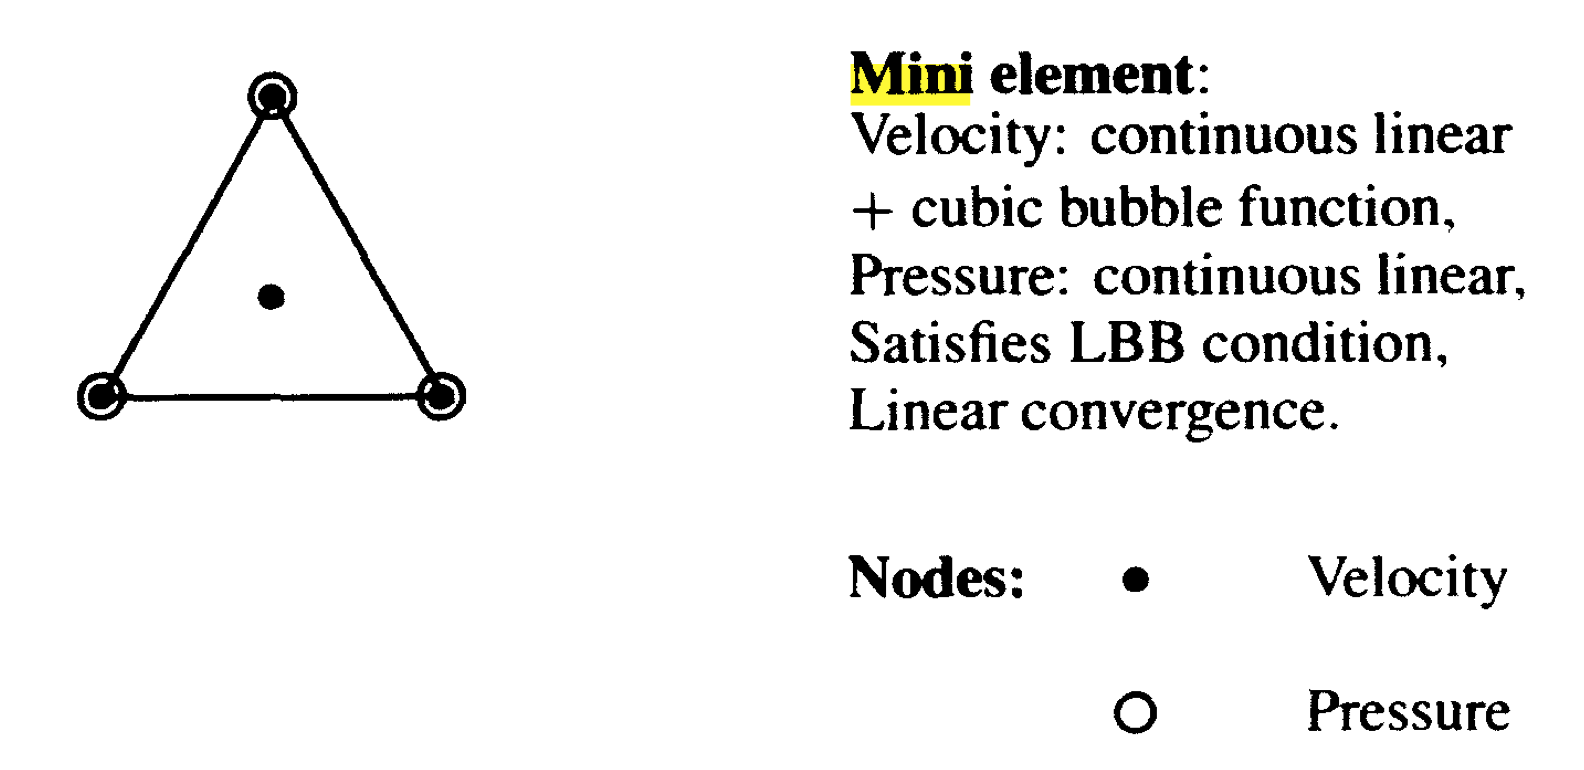
\includegraphics[width=8cm]{images/mini/minielement}\\
{\captionfont Figure taken from Donea and Huerta \cite{dohu03}}
\end{center}

\begin{remark}
Note that \cite{frol03} propose an equal-order-linear-continuous velocity-pressure variables which is enriched 
with velocity {\it and} pressure bubble functions to model the Stokes problem. They show by static condensation that
these bubble functions give rise to a stabilized method involving least-squares forms of the momentum and of the
continuity equations. In some cases their approach recovers the MINI element. Also check \cite{gamt08}.
\end{remark}

\begin{remark}
According to Braess\cite{braess}, since the support of the bubble is restricted to the element, 
the associated variable (dofs living on the bubble) can be eliminated from the resulting 
system of linear equations by static condensation. \index{general}{Static Condensation}
Also, the MINI element is cheaper than the Taylor-Hood element but it is commonly accepted
that it yields a poorer approximation of the pressure.
\end{remark}

The 3D MINI element is not very common but it is used for instance in \cite{pico98}.
It is also said to be LBB stable in \cite[p180]{reddybook2}.

\begin{center}
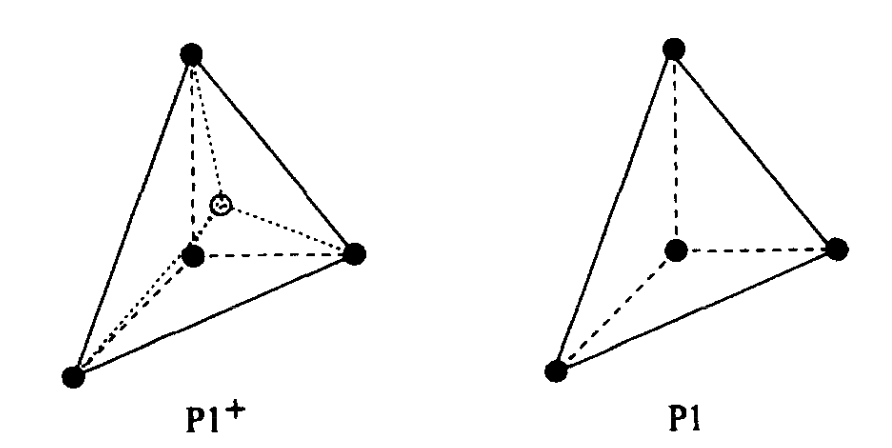
\includegraphics[width=10cm]{images/mini/mini3D}\\
{\captionfont Velocity and pressure nodes for the 3D MINI element, taken from \cite{pico98}}
\end{center}

Note that this element is used in \cite{brwr00} in the context of Arbitrary Lagrangian Eulerian 
finite element analysis of free surface flows.
Also used in Zlotnik et al (2007) \cite{zldf07} for suduction with X-FEM technique.







%----------------------------------------------------------------------
\subsubsection{The quadratic velocity - linear pressure triangle ($P_2\times P_1$)}

From \cite{segal}: \say{Taylor-Hood elements \cite{taho73} 
are characterized by the fact that the pressure is continuous in the region $\Omega$. 
A typical example is the quadratic triangle (P2P1 element).
In this element the velocity is approximated by a quadratic polynomial and the pressure by a
linear polynomial. One can easily verify that both approximations are continuous over 
the element boundaries.}
It can be shown, Segal (1979), that this element is admissible if at least 3 elements 
are used. The quadrilateral counterpart of this triangle is the $Q_2\times Q_1$ element.
Reddy and Gartling \cite[p179]{reddybook2} also report this element to be LBB stable.

\Literature: \cite{scan85,lejx14,cump20}


%----------------------------------------------------------------------
\subsubsection{The Crouzeix-Raviart triangle ($P_2^+\times P_{-1}$)}
\label{sec:crouzeix-raviart}

Since the $P_2\times P_{-1}$ pair is not LBB stable \cite[p179]{reddybook2}, 
it is enhanced by a cubic bubble and is therefore called $P_2^+\times P_{-1}$. 

This element was first introduced in \cite{crra73}.
It is the element used in the MILAMIN code \cite{daks08}.
It is a seven-node triangle with quadratic velocity shape 
functions enhanced by a cubic bubble function and discontinuous linear interpolation for 
the pressure field \cite{cuss86}. 
This element is LBB stable and no additional stabilization techniques are required\cite{elsw}.
The '+' in its name stands for the bubble while the '-' stands for the discontinuous
character of the pressure field: once again, it is $P_1$ over the element, but discontinuous
across element edges.

\begin{remark}
Cuvelier et al, 1986 \cite{cuss86} recommend a 6-point or 7-point quadrature rule for this element.
\end{remark}

\begin{remark}
Segal \cite{segal} explains 
for output purposes (printing, plotting etc.) the discontinuous pressures are averaged 
in vertices for all the adjoining elements. See also Fig. 7.3 of \cite{cuss86}.
\end{remark}

\begin{remark}
The simplest Crouzeix-Raviart element is the non-conforming linear triangle 
with constant pressure ($P_1\times P_0$) \cite{cuss86}. 
\end{remark}

It is worth noting that this element has more degrees of freedom  than the 
Taylor-Hood element for the same order of accuracy. However, since the 
bubble can be eliminated, one can design a modified version of this element.
\todo[inline]{Check Cuvelier book chapter 8 for modified element}


\begin{remark}
I have once asked the (main) author of MILAMIN why he chose this element, for 
example over the $P_2\times P_1$. His answer is as follows:
"Elements with continuous pressure  are incapable of converging in the Linf 
norm for mechanical problems exhibiting pressure jumps such as the inclusion-host setup. 
During my MSc and PhD I was focusing on sharp heterogeneities, so this is why I decided 
to choose $P_2^+\times P_{-1}$. 
You will see that it is also easy to invert the pressure mass matrix for such elements, 
which is really useful (both for the augmentation and preconditioning)."
\end{remark}

This element is used by Poliakov and Podlachikov \cite{popo92} to study the deformation of the surface above a rising diapir. Note that they actually use a "13 point integration formula (Hughes
1987) for calculation of the stiffness matrix was used in order
t o conserve detailed information from the marker field in
the coarse FEM mesh". 
It is also used in \cite{anmp15} in the context of a new free-surface stabilization scheme. 
It is the element used in LaCoDe \cite{demh19}.






%-----------------------------------------------------------------
\subsubsection{The Rannacher-Turek element - rotated $Q_1\times P_0$} \label{ss:RTq1p0}
\index{general}{$\tilde{Q}_1\times P_0$}
\index{general}{Korn's inequality}
\index{general}{Rannacher-Turek element}
\index{general}{Nonconforming element}

This element is the natural quadrilateral analogue
of the well–known triangular Stokes element of Crouzeix-Raviart \cite{crra73}.
This element is sometimes called $Q_1^{rot} \times Q_0$ or the Rannacher-Turek element 
\cite[Section 3.6.5]{john16}.
This rectangular nonconforming \cite{crfa89} element is termed the rotated $Q_1$ element 
because of the fact that $r^2-s^2$ can be generated from $rs$ (occurring in the bilinear $Q_1$ 
element) by a rotation of 45$\degree$ \cite[p93]{chen}.
The velocity approximation is achieved by rotated dim-linear functions that have 
continuous degrees of freedom on
the faces of the mesh cells as we have seen in Section~\ref{ss:rq1}.
This element was introduced in Rannacher \& Turek (1992) \cite{ratu92} 
has been proven to satisfy the inf-sup condition. It has been studied comprehensively in Schieweck 
(1997)\footnote{Habilitation thesis in German}, \cite{shzh06} and in Turek \cite{ture94,ture96}.
Superconvergence properties have also been reported \cite{misx06,misx07}.
It has been used in 2D \cite{maky17} and 3D \cite{klll96,gekm08} and forms the basis of the FeatFlow 
software\footnote{\url{http://www.featflow.de/en/index.html}}. 
It is used in the PhD thesis of Gastaldo \cite{gast07} and Ouazzi \cite{ouaz05}.
It has been 
successfully coupled to multigrid solvers \cite{chos98,tuos02}.
This element has been compared to the stabilised $Q_1\times P_0$ element \cite{lisi12}.
It is mentioned in \cite{hans11}

It essentially comes in two flavours, the Middle Point (MP) and the Mid Value (MV) one.

\begin{remark} 
John \cite{john16} explains that: "For the point-value-oriented non-conforming finite element spaces (MP), 
the value of the Dirichlet boundary
condition in the barycenter of the faces at the boundary is taken. Using the mean-
value-oriented spaces (MV), one computes the integrals of the boundary condition on
these faces and normalizes with the area of the faces to set the boundary values.
In the case of homogeneous Dirichlet boundary conditions, the boundary values
computed in both ways are zero."
\end{remark}

\begin{remark} 
John also makes a very important point: "There are also unmapped (non-parametric) versions of 
these finite element spaces, which define the polynomials directly on the mesh cell K. It is shown in Rannacher
and Turek (1992) \cite{ratu92} that these versions are inf-sup stable on more general meshes than
the mapped (parametric) version of the $Q_1^{rot}\times Q_0$ finite element, e.g., on strongly
nonuniform meshes. Considering all four types of $Q_1^{rot}\times Q_0$ finite elements, the
optimal order of convergence on perturbed meshes is achieved only by the mean-
value-oriented version of the unmapped $Q_1^{rot}\times Q_0$   finite element.
\end{remark}

Mahmood et al \cite{maky17} mention a very important fact: "The chosen nonconforming element requires
additional stabilization for handling the deformation tensor formulation due to missing Korn’s inequality 
\cite{horg95,knob00}.
To this end we employ the standard edge oriented stabilization \cite{tuos02,tuou07} in our simulations."
This is a rather unfortunate fact that although LBB stable this element needs an additional 
term in the weak form (see Turek et al (2002) \cite{tuos02}) 
so as to suppress parasitic velocity modes when the div-grad formulation 
of the Stokes equation is used (as opposed to the Laplace formulation -- see \cite[Section 6.5.2]{dohu03}).




%\Literature 









%----------------------------
\subsubsection{Other elements}

\begin{itemize}
\item $P_1\times P_0$: example 3.70 in \cite{john16}, also \cite{john98}. \index{general}{$P_1\times P_0$}
\item $P_1\times P_1$ stabilised \cite{nosi98,tasu00}
\item Q2P0: \index{general}{$Q_2 \times P_0$}: 
Quadratic velocities, constant pressure. The element satisfies the inf-sup condition, but the constant pressure assumption may require fine discretisation.

\item Q2Q2: This element is never used, probably because a) it is unstable, b) it is very costly. 
There is one reference to it in \cite{hufb86}.
\item Q1P-1 Bilinear velocities,  piecewise linear discontinuous polynomial pressure.
\item See Fortin \cite{fort81} for various stable low order elements
\item Stable cheapest nonconforming finite elements for the Stokes equations \cite{kiys16}
\item Q1Q1 + nonconforming null edge average \cite{fros07}
\item P3-P2 mentioned in \cite{sten90}   \index{general}{$P_3\times P_2 element$}

\end{itemize}

%.........................................................................
\subsubsection{A note about incompressibility and standard mixed methods}

What follows is nicely explained and demonstrated in John et al \cite{jolm17}. In their 
example 1.1 they look at the velocity error of benchmark VJ2 (see Section~\ref{mms9}) 
which analytical solution is a zero velocity field. They show that for the MINI, 
Taylor-Hood and Crouzeix-Raviart triangular elements the velocity error grows 
with the magnitude of the rhs. They also make this statement:
\say{
there are important applications, e.g., natural
convection problems, where the pressure is larger than the velocity by orders
of magnitude. In such situations, one cannot expect to compute accurate
velocity fields with classical mixed methods, at least for low order methods.
}




